\section{Pneumatic System}

The goal of this section is to describe the design of the pneumatic actuation system intended to meet the goals outlined in Sec. \ref{sec:goals_transmission}. The background of the transmission and transmission control system used in the 2009 Formula SAE vehicle was discussed in Sec. \ref{sec:background_transmission}. The new design for this project improves upon this previous generation by targetting several of the noted deficiencies, while reusing specific portions that worked well.

The possibility of using a fully electronic actuation system, with geared DC motors, was carefully considered: the control of such a system would be far simpler, as linear approximate models of DC motors are readily available. Reasonably priced gearhead motors from several suppliers were investigated. It was determined however that to meet the torque and duty-cycle requirements of transmission actuation, any suitable fully electronic system would be far heavier than the pneumatic equivalent.

After deciding to keep a pneumatic actuation system, an improved valving scheme was proposed for the clutch, and sources of feedback were determined so that a closed-loop controller could be designed. Several academic papers were sourced that describe successuful methods of pneumatic actuator control. \Citet{pneumatic_actuator} and \citet{adaptive_pneumatic} both use an electronically adjustable proportioning valve and a dual-acting cylinder. Proportioning valves are expensive (approximately \$300 from local suppliers) in comparison with binary solenoid valves (under \$50.)

Another approach by \citet{accurate_position} uses PWM signalled 3-way solenoid valves to control the air in and out of both sides of a dual-acting cylinder. By varying the duty cycle of the input signals, they were able to modulate the effective mass air flow rate through the cylinder ports: with the valve open, air would tend to flow from the high-pressure source into the cylinder, and with the valve closed, air would flow from the pressurized cylinder out through the exhaust port of the valve. This valving scheme allowed for a high degree of positional accuracy, however a large amount of air would be consumed during operation, as air is constantly being exhausted.

\subsection{Subsystem Overview}

A diagram of the mechanical portion of the pneumatics system can be seen in Fig. \ref{fig:pneumatics_design}. As in the previous design, an on-board compressed air tank is fitted with a pressure regulator, which regulates the system pressure to approximately $\unit{0.8}{\mega\pascal}$. Four solenoid valves controlled with signals $U_U$, $U_D$, $U_A$, and $U_B$ control the flow of air to and from 2 pneumatic actuators.

\begin{figure}[H]
\centering
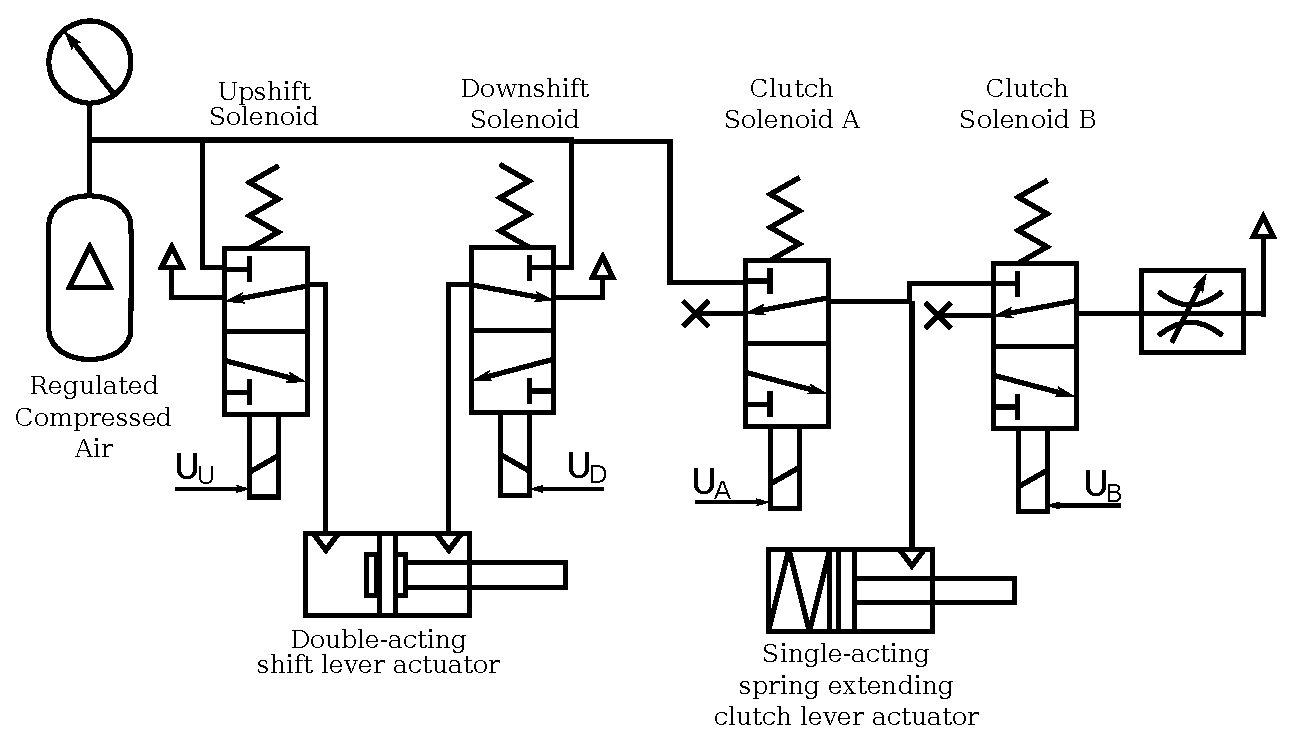
\includegraphics[scale=0.5]{design/figures/pneumatics}
\caption{Transmission control pneumatics design.}
\label{fig:pneumatics_design}
\end{figure}

\subsubsection{Clutch Actuation}
\nomenclature{PWM}{Pulse Width Modulation}
\nomenclature{$U_U$, $U_D$}{Output signals from the transmission controller to the upshift and downshift solenoids.}
\nomenclature{$U_A$, $U_B$}{Pulse width modulated output signals from the transmission controller to clutch solenoids A and B.}

The three approaches described in \cite{pneumatic_actuator, adaptive_pneumatic, accurate_position} considered the possibility of a highly dynamic load on the actuator, however the load seen by the clutch actuator is in fact far more predictable than the loads they expected, and only uni-directional. Since the vehicle is only equipped with a limited supply of air, conservation is a concern. Taking these factors into account, a sigle-acting cylinder with a return spring is specified for the clutch, and we propose a new valving scheme  that allows a degree of controllability over actuator while conserving as much air as possible.

The cylinder visible on the right of Fig. \ref{fig:pneumatics_design}, actuates the clutch lever. Precise control of the clutch is accomplished with fast solenoid valves \emph{Clutch Solenoid A} and \emph{Clutch Solenoid B}. These valves are signalled with \emph{Pulse Width Modulated} (PWM) signals, which modulate the average mass air flow rate into and out seperately of the cylinder. Position feedback for the clutch cylinder is provided by a combination of an internal magnet on the piston in the cylinder, and a magnetic sensing membrane potentiometer.

Both clutch solenoids are shown as 3-way (with exhaust ports) valves in Fig. \ref{fig:pneumatics_design}, however the valves are used in a 2-way configuration: the exhaust ports are closed off with a plug. This results in the following operation:
\begin{enumerate}
  \item When the pulse width modulated control signal $U_A$ to Clutch Solenoid A is non-zero, the valve will open, and air will flow into the cylinder at a rate proportional to the duty cycle, disengaging the clutch.
  \item When pulses no longer arrive at Clutch Solenoid A (or the duty cycle of $U_A$ approaches 0), the valve remains closed, and any air in the cylinder is trapped. The clutch maintains is position.
  \item When the pulse width modulated control signal $U_B$ to Clutch Solenoid B is non-zero, the valve will open, and any pressure differential between the cylinder and atmosphere will cause air to flow out of the cylinder to atmosphere at a rate proportional to the duty cycle. The clutch springs and the cylinders' internal spring work to return the actuator position to rest, and the clutch engages.
\end{enumerate}

An additional adjustable flow rate control valve (visible on the far right in Fig. \ref{fig:pneumatics_design}) was added to the design to allow additional tuning for during clutch engagement. Coupled with a suitably tuned closed-loop controller, the electro-pneumatic actuation system will meet the controllability requirements outlined in \ref{sec:goals_transmission}. In the clutch operation, since the fill and exhaust operations are seperately controlled with two valves (compared to the use of one 3-way valve in \cite{accurate_position}), no air is wasted in disengaging the clutch and holding the position.

\subsubsection{Shift Actuator}

The shift lever does not require the same level of control as the clutch, and as such the design of the valving has not changed over previous implementations: two binary valves will be used with a dual-acting cylinder. The addition of a feedback path from the transmission indicating the currently selected gear in the transmission will improve the controller.

The first actuator, visible on the left of Fig. \ref{fig:pneumatics_design}, actuates the shift lever between 3 different positions: upshift, downshift, and rest-state. The transmission spring-loads the lever to automatically return to the rest-state, which we have set up to be half-way through the actuator stroke. Individually applying pressure to one port will pull the lever up, and to the other port, down.

Current gear position is determined with a potentiometer that is mechanically linked to the shift drum. Control and timing are generated by the controller, and respond to requests from the driver.